\documentclass[10pt,letterpaper]{article}
\usepackage[margin=.82in]{geometry}
\usepackage[T1]{fontenc}\usepackage{lmodern,graphicx,booktabs,amsmath,xcolor,hyperref,xurl,caption,fancyhdr}
\hypersetup{colorlinks=true,urlcolor=teal,linkcolor=teal,pdftitle={Compare employment on a consistent population base},pdfauthor={James Jean}}
\pagestyle{fancy}\fancyhf{}\fancyhead[L]{\small Japan employment versions / Study 33}\fancyhead[R]{\small Independent measurement audit}\fancyfoot[C]{\thepage}
\setlength{\headheight}{14pt}\setlength{\parindent}{0pt}\setlength{\parskip}{6pt}\captionsetup{font=small,labelfont=bf,hypcap=false}
\begin{document}
{\small\color{teal} REGIONAL STATISTICS / VERSION CONSISTENCY\par}
\vspace{7pt}{\LARGE\bfseries Compare employment on a\par consistent population base\par}
\vspace{7pt}James Jean \hfill 30 October 2026

\textbf{Decision.} Before interpreting an employment-growth signal, check that the current count and its comparison count use the same dataset version. Official historical counts can be revised when the population benchmark changes. Mixing a newer numerator with an older denominator can produce a different growth direction without either input being an invented number.

\textbf{Measured result.} In 72 later region-month comparisons from Southern-Kanto and Kinki, Japan, the authored mixed-version calculation differs from the current coherent calculation by a mean absolute 0.327 percentage points and a maximum 0.577 percentage points. There are 4 strictly opposite published growth signs; 2 remain opposite under conservative count-rounding enclosures. These are finite retrospective comparisons, not an error rate for a live dashboard.

\begin{center}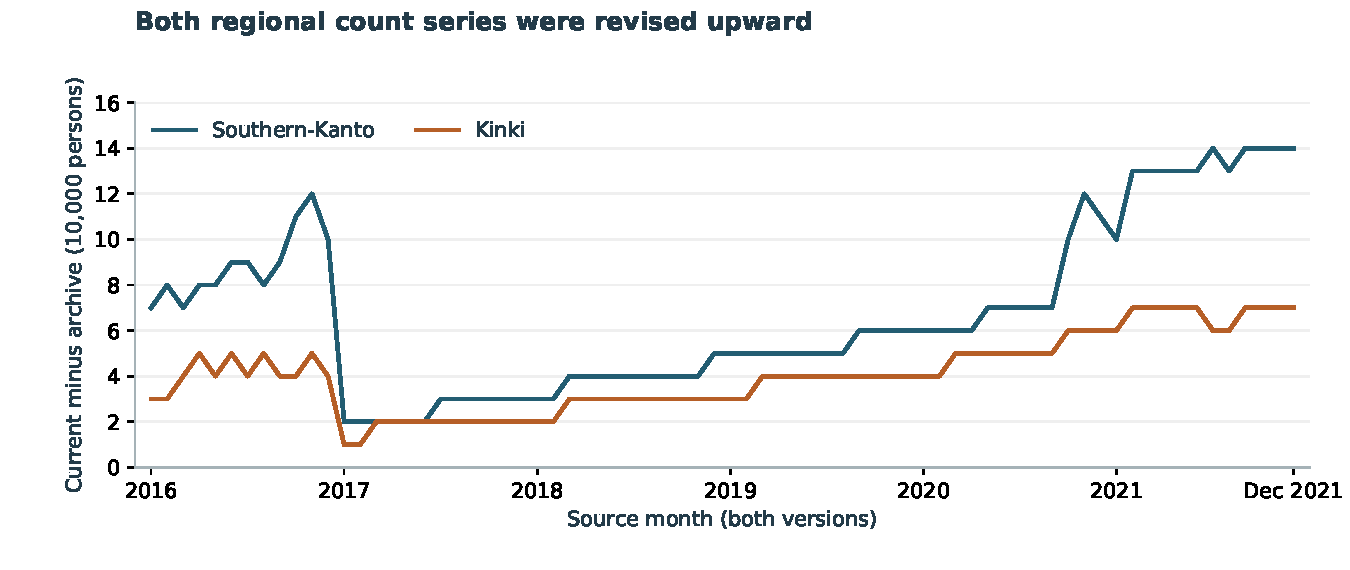
\includegraphics[width=\linewidth]{images/count_revisions.pdf}\end{center}
\captionof{figure}{Current historical counts minus the official pre-2022 archive, in ten thousand persons, for the fixed source window. Both regions are revised upward in every selected month. A level revision is not itself a change in true employment. The differences compare complete retrieved versions and do not identify the effect solely of the 2020 Census rebase. Source: Statistics Bureau, Japan; processed by this study.}

\textbf{Practical recommendation.} Reload the comparison history when accepting a revised count series, preserve its version and reject incompatible pairs. Treat near-boundary values as rounding-ambiguous. Sampling uncertainty remains additional and unestimated here. Employment counts describe people employed under a reference-week definition; they do not establish vacancies, recruiting demand, a causal policy effect or measured business savings.
\newpage
\section*{1. Which numbers are being compared?}
The Statistics Bureau's benchmark page records the move to a 2020-Census population base in January 2022 for Basic Tabulation. Earlier counts were replaced by retroactive or intercensal-adjusted values. The linked archive explicitly preserves original series before that revision. The current historical table 1-e-1 contains the corresponding monthly regional reference series. Publisher notes warn that annual reports retain publication-time figures while historical tables are revised, and that these monthly regional reference estimates have lower precision than national results [1--4].

The fixed cohort contains 288 count cells: 72 months for each of 2 regions in 2 versions. Source months are January 2016 through December 2021. The comparison window starts one year later. Development uses 2017--2018, and the later check uses 2019--2021. All planned cells are present, positive integer native numeric cells without formulas; no missing month, imputation or conflicting key is hidden.

\begin{center}\small
\begin{tabular}{@{}p{.23\linewidth}p{.70\linewidth}@{}}\toprule
Identity & Binding retained in both sources\\\midrule
Southern-Kanto & Saitama, Chiba, Tokyo and Kanagawa\\
Kinki & Shiga, Kyoto, Osaka, Hyogo, Nara and Wakayama\\
Employment concept & \textit{Employed person}, not the adjacent \textit{Employee} column\\
Population/sex & Aggregate regional total; no sex subgroup is selected\\
Unit/adjustment & Ten thousand persons; original monthly reference counts\\
Archive version & Before 2020-Census benchmark revision, captured in 2026\\
Current version & Historical table retrieved October 30, 2026\\\bottomrule
\end{tabular}\end{center}

\textbf{The label matters.} The Japanese header is retained beside the source's English \textit{Employed person} label. Under the official definition, employed persons include people who worked for pay or profit, qualifying unpaid family workers, and people with jobs temporarily not at work. The adjacent employees-only column is a different concept. A translation does not justify replacing one with the other. This release does not test industry-classification crosswalks or estimate a prefecture panel.

\textbf{Version limits.} The archive is an official pre-2022 benchmark version, not proof of the first delivered value for every historical month. The current file is the retrieved 2026 historical version, not a frozen March 2022 release. Differences can include cumulative revisions. No next-release forecast, isolated census-rebase effect or prospective vintage backtest is established.

\textbf{Source handling.} Exact request URLs, capture times, hashes, cell coordinates, visible Japanese/English month labels and native count tokens are retained. A raw OOXML reader initially appended Japanese phonetic annotations to date labels and stopped before projection or scoring. The targeted correction excludes those annotation runs from displayed text. Independent Openpyxl/calendar parsing and separate raw-token checks reconcile all selected cells. Source originals were read without modification or recalculation; complete workbooks and publisher documents remain private.
\newpage
\section*{2. Coherent growth, a splice and rounding}
Let $O_t$ be the archived count and $N_t$ the current historical count for the same region and month. Retain three exact comparisons:
\[
g_O=O_t/O_{t-12}-1,\qquad g_N=N_t/N_{t-12}-1,\qquad g_M=N_t/O_{t-12}-1.
\]
The mixed calculation $g_M$ is an authored ingestion error, not an observed organizational incident. The reference $g_N$ is coherent within one retrieved version; it is not ground truth for unobserved true employment. Archive-versus-current differences and mixed-versus-current discrepancies are separate outputs. Reported discrepancies are percentage points: $100(g_j-g_N)$.

For a positive displayed count $x$, use the conservative closed rounding enclosure $[x-0.5,x+0.5]$ in the native ten-thousand-person unit. For a numerator $a$ and denominator $b>0.5$:
\[
L=(a-0.5)/(b+0.5)-1,\qquad U=(a+0.5)/(b-0.5)-1.
\]
Only $L>0$ certifies positive growth, and only $U<0$ certifies negative growth; otherwise the sign is ambiguous. These are rounding enclosures, not confidence intervals or a model of sampling error. For a fixed absolute-growth threshold $h$, certify an alert if $L\ge h$ or $U\le-h$, certify no alert if $L>-h$ and $U<h$, and otherwise retain ambiguity.

\textbf{Worked later example: Kinki, November 2020.} Counts below are in ten thousand persons. The source comparison month is November 2019. A newer numerator divided by the older comparison count flips the sign. Both intervals still exclude zero in opposite directions; this does not resolve sampling uncertainty.
\begin{center}\small\begin{tabular}{@{}lrrrrr@{}}\toprule
Calculation & Numerator & Denominator & Growth(\%) & Lower(\%) & Upper(\%)\\\midrule
Archive coherent & 1,066 & 1,070 & -0.374 & -0.467 & -0.281 \\
Current coherent & 1,072 & 1,074 & -0.186 & -0.279 & -0.093 \\
Authored mixed & 1,072 & 1,070 & 0.187 & 0.093 & 0.281 \\
\bottomrule\end{tabular}\end{center}

\textbf{Earlier implementation check.} There is no learned model, threshold optimization or comparator selection. Both illustrative thresholds, 0.5\% and 1\%, and all comparisons remain visible. The following development results were produced before committing 24 dependency hashes and before later decision summaries. Source completeness inspection covered the full cohort; no analyst-blindness or untouched-schema claim is made.
\begin{center}\small\begin{tabular}{@{}lrrrrrr@{}}\toprule
Vs.current & Pairs & Mean abs.pp & Max abs.pp & Sign diff. & Opposite & Robust\\\midrule
Archive & 48 & 0.185 & 0.473 & 2 & 1 & 0 \\
Mixed & 48 & 0.300 & 0.627 & 3 & 1 & 0 \\
\bottomrule\end{tabular}\end{center}
``Sign diff.'' includes a point estimate of zero versus a nonzero value. ``Opposite'' requires strictly opposite point signs. ``Robust'' further requires opposite signs throughout both rounding enclosures. Neighboring months share survey and revision information; the rows are not independent trials.
\newpage
\section*{3. Later comparisons across both regions}
\begin{center}\small\begin{tabular}{@{}llrrrrrr@{}}\toprule
Region & Vs.current & Pairs & Mean abs.pp & Max abs.pp & Sign diff. & Opp. & Robust\\\midrule
Southern-Kanto & Archive & 36 & 0.150 & 0.344 & 1 & 1 & 1 \\
Southern-Kanto & Mixed & 36 & 0.278 & 0.577 & 2 & 1 & 0 \\
Kinki & Archive & 36 & 0.123 & 0.285 & 5 & 0 & 0 \\
Kinki & Mixed & 36 & 0.375 & 0.566 & 7 & 3 & 2 \\
All & Archive & 72 & 0.136 & 0.344 & 6 & 1 & 1 \\
All & Mixed & 72 & 0.327 & 0.577 & 9 & 4 & 2 \\
\bottomrule\end{tabular}\end{center}
\textbf{Interpretation.} Mixing versions creates larger average discrepancies than comparing two coherent versions in this fixed later cohort. The two comparisons answer different questions: a coherent archive/current contrast measures a change in published historical estimates; the authored splice additionally changes the comparison basis within a growth calculation. Neither estimates true employment error or a causal effect of a population census.

\begin{center}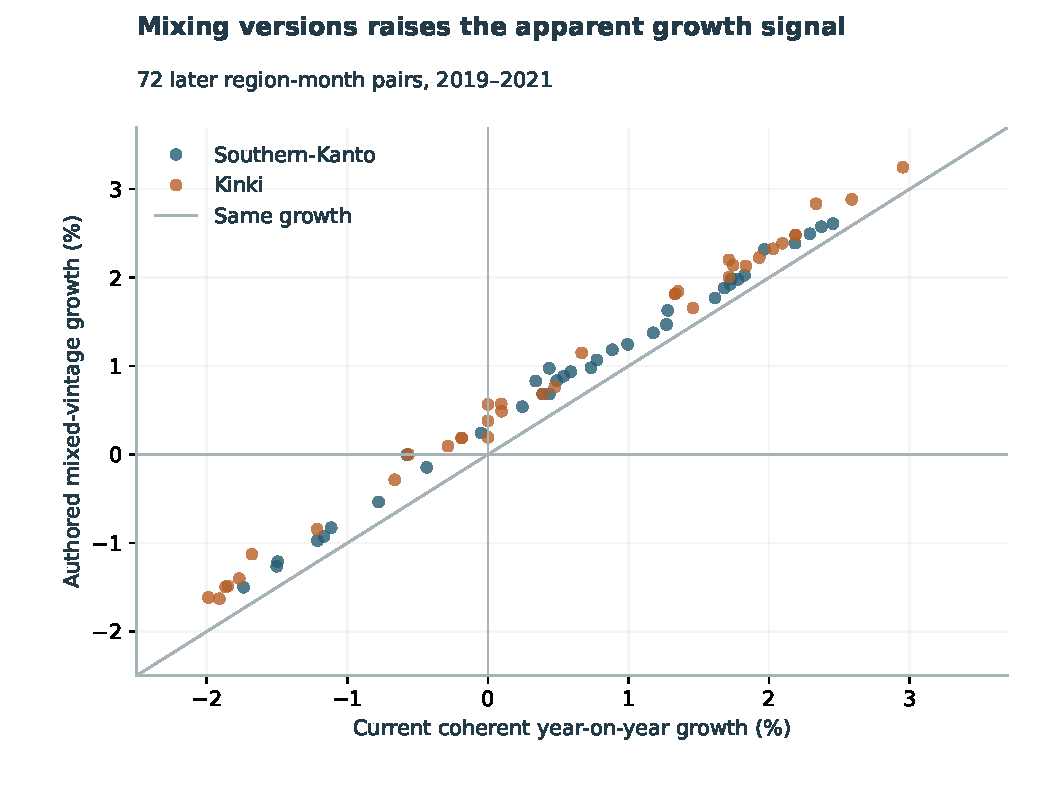
\includegraphics[width=.80\linewidth]{images/growth_splice.pdf}\end{center}
\captionof{figure}{Each point is one later region-month pair. The diagonal represents identical growth. Upward displacement comes from replacing the denominator with the older count while retaining the current numerator. The common current numerator and the source-month overlap mean points are dependent. Overlapping markers are retained, not jittered or treated as fewer observations.}

The source counts are revised upward in both regions throughout the selected window, so this splice has an upward direction here. That finite pattern is not a universal rule about revisions. The two rounding-robust opposite-sign cases occur in Kinki in November and December 2020. Ambiguous point reversals remain separately reported rather than being promoted into certified reversals.
\newpage
\section*{4. Thresholds need an ambiguity state}
\begin{center}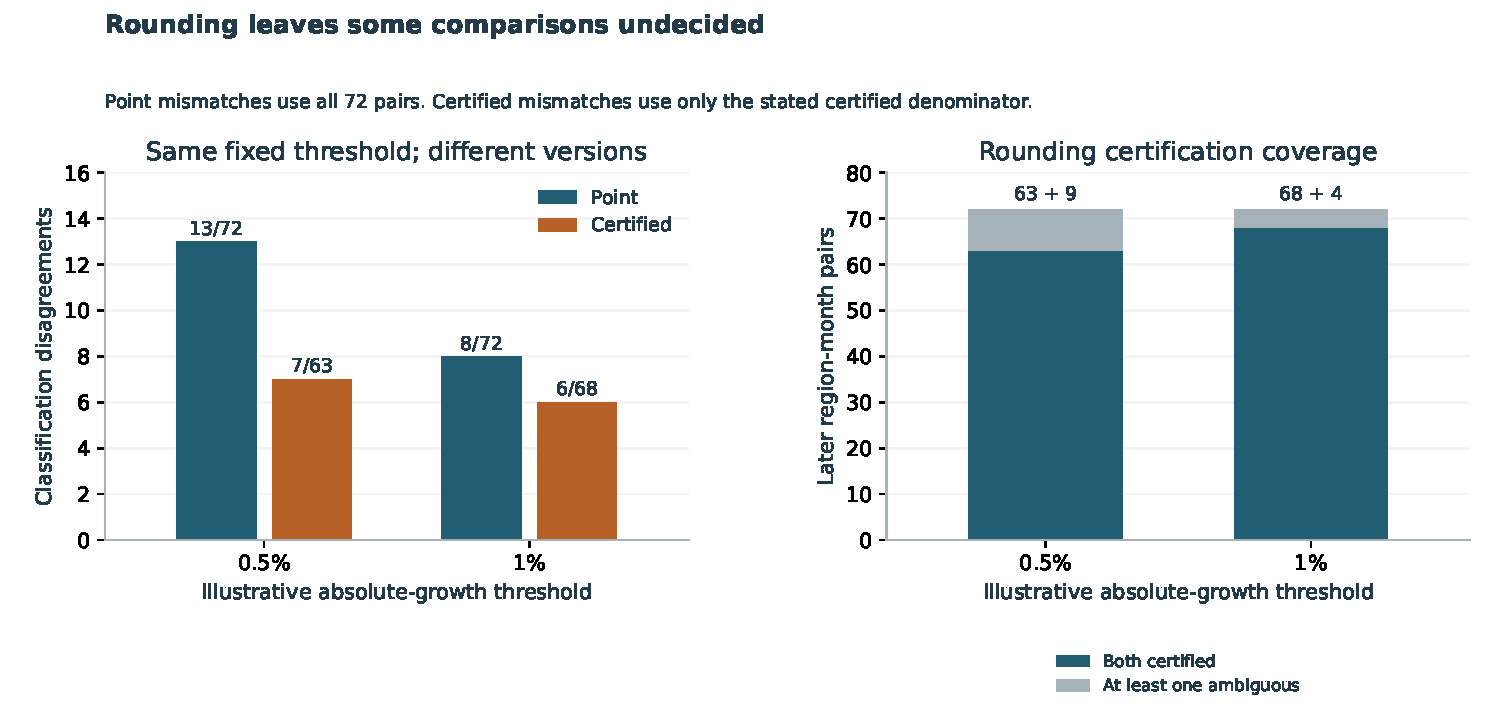
\includegraphics[width=\linewidth]{images/threshold_coverage.pdf}\end{center}
\captionof{figure}{Later mixed-versus-current classifications at both fixed illustrative thresholds. Point mismatches use all later pairs. A certified mismatch is counted only when both compared rounding enclosures have a certified classification. The remaining pairs are ambiguous, not counted as correct non-alerts. The chart does not estimate real alert precision or select an operating threshold.}

\begin{center}\small\begin{tabular}{@{}lrrrr@{}}\toprule
Vs.current & Threshold(\%) & Point mismatches & Both certified & Certified mismatches\\\midrule
Archive & 0.5 & 5 & 66 & 2 \\
Archive & 1.0 & 1 & 70 & 0 \\
Mixed & 0.5 & 13 & 63 & 7 \\
Mixed & 1.0 & 8 & 68 & 6 \\
\bottomrule\end{tabular}\end{center}

\textbf{Implementation exercise.} Build a small version guard before doing arithmetic. Geography, concept, sex scope, adjustment, native unit and dataset version must match, and the denominator must be for the same month one year earlier. Missing or conflicting identity returns unavailable with a reason. The supplied authored counts of 101 and 100 produce exact growth of 1/100, but their rounding enclosure includes zero. They are fixture values, not Japanese source records.

The local CLI and reference solution implement that boundary without source access, accounts or paid services. A matching version string is a declared input contract; the guard cannot authenticate a source or independently prove that two files share a population base. In a real pipeline, retain publisher/version metadata and source arrivals, reload historical comparison values with revised series, and reconcile ambiguous mappings explicitly.

\textbf{What this exercise does not establish.} The benchmark has no observed hiring-incident labels, user trial or deployment. Its thresholds are fixed examples, not calibrated business decisions. It does not show that any real employer, dashboard or public agency made the authored splice error, nor that rejecting it generated measured savings.
\newpage
\section*{5. Evidence, limits and next step}
Independent original-cell reconciliation passes 2,600 finite conditions. Exact SQLite/integer/Fraction reconstruction passes 4,930 development conditions and 6,922 later conditions. The 44 finite fixtures cover source identities, missing/zero values, conflicting keys, era/Gregorian month labels, year lags, rounding boundaries, threshold ambiguity and the local version guard. Perfect results on these finite fixtures do not establish universal correctness or production readiness.

The committed freeze records source projection, definitions, code, checks, fixtures and development exports before later summaries. No parameter is fitted and neither threshold is selected. Offline replay uses a clean full-history clone, writes regenerated numerical exports to separate paths, compares exact CSV fields and JSON content, and checks that frozen originals remain unchanged. Original-workbook reconciliation is a separate optional check requiring the captured byte-identical files. A newly downloaded workbook may be a different version.

\textbf{Presentation and disclosure.} Original figures have source queries and actual SVG-geometry checks; the manuscript retains a numerical display ledger and LaTeX source. Source metadata and the national benchmark example were visible before cohort capture. Header binding and source qualification occurred after capture. No analyst-blindness, untouched-schema, next-release forecast, new estimator or scientific-priority claim is made. The earlier source-reader failure and visual overlap check are retained privately; neither was corrected by changing a source value or threshold.

\textbf{Limits.} Two regional reference series do not represent every prefecture or an industry panel. These monthly estimates have reduced sampling precision; rounding enclosures do not quantify it. The observations share months, surveys and benchmark revisions. Historical version changes are not causal effects on actual employment. No trained model, R implementation, vacancy-demand estimate, live error rate, measured financial impact or peer review is established. This is an independent program manuscript, with formal-publication projects excluded.

\textbf{Next evidence.} For an operational dashboard, first preserve source-version lineage and check the historical reload process. Then measure observed version conflicts and reconciliation workload against independently labeled ingestion incidents, while using the publisher's sampling-error guidance for substantive regional interpretations. Those records are needed before choosing an operating threshold or claiming a practical error-rate improvement.

\section*{Primary sources and code}
\small
[1] Statistics Bureau, Japan. \href{https://www.stat.go.jp/english/data/roudou/220201/index.html}{2022 revision of benchmark population}, including the linked pre-revision workbook and benchmark-method note. Published March 4, 2022; revised May 13, 2022. The current study captures exact objects on October 30, 2026.

[2] e-Stat, Labour Force Survey, Basic Tabulation, \href{https://www.e-stat.go.jp/en/stat-search/files?cycle=0\&tclass=000001226526}{historical table index}, table 1-e-1, monthly Southern-Kanto/Kinki reference results. Exact download URL and hashes are retained in the repository source receipt.

[3] Statistics Bureau, \href{https://www.stat.go.jp/english/data/roudou/note.html}{Notes on the results}; \href{https://www.stat.go.jp/english/data/roudou/pdf/definite.pdf}{Concepts and Definitions}; \href{https://www.stat.go.jp/english/data/roudou/result.html}{The Survey Results}.

[4] Statistics Bureau, \href{https://www.stat.go.jp/english/info/riyou.html}{website-use policy}; e-Stat, \href{https://www.e-stat.go.jp/en/terms-of-use}{Terms of Use}. Source numerical facts are attributed; this study's projection/calculations are processed content, with no government endorsement. Third-party exceptions remain applicable.

Code, complete exports, source hashes, figures and exercise: \url{https://github.com/S3R3Bii/japan-employment-vintages}.
\end{document}
